\documentclass[border=5pt]{standalone}
\usepackage{tikz}
\usetikzlibrary{positioning,arrows.meta,decorations.markings,bending}

\begin{document}
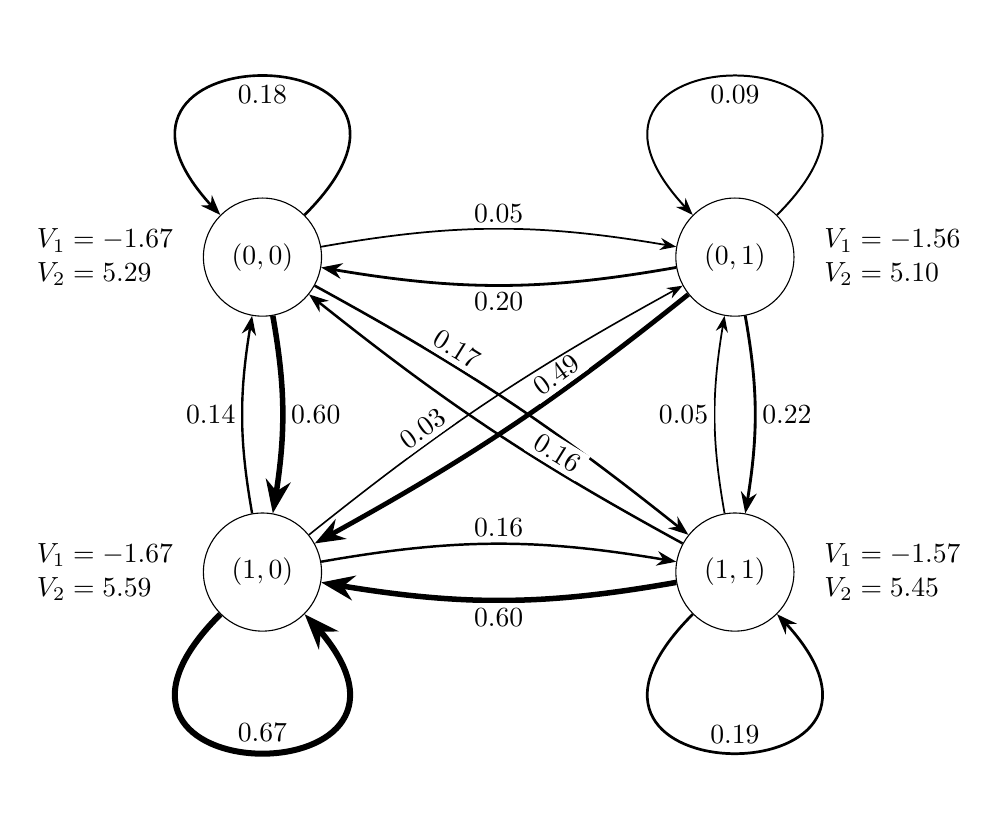
\begin{tikzpicture}[>=Stealth]

  % Define states
  \node[circle, draw, minimum size=1.5cm] (s00) at (0,0) {$(0,0)$};
  \node[circle, draw, minimum size=1.5cm] (s01) at (6,0) {$(0,1)$};
  \node[circle, draw, minimum size=1.5cm] (s10) at (0,-4) {$(1,0)$};
  \node[circle, draw, minimum size=1.5cm] (s11) at (6,-4) {$(1,1)$};

  % Value functions
  \node[align=left] at (-2,0) {$V_1=-1.67$ \\ $V_2=5.29$};
  \node[align=left] at (8,0) {$V_1=-1.56$ \\ $V_2=5.10$};
  \node[align=left] at (-2,-4) {$V_1=-1.67$ \\ $V_2=5.59$};
  \node[align=left] at (8,-4) {$V_1=-1.57$ \\ $V_2=5.45$};

  % Transitions
  \path[->,line width=0.95pt] (s00) edge[out=45,in=135,looseness=8] node[auto,pos=0.5] {0.18} (s00);
  \draw[->,line width=0.63pt] (s00) edge[bend left=10] node[above,fill=white,inner sep=2pt,pos=0.50] {0.05} (s01);
  \draw[->,line width=1.99pt] (s00) edge[bend left=10] node[right,fill=white,inner sep=2pt,pos=0.50] {0.60} (s10);
  \draw[->,line width=0.93pt] (s00) edge[bend left=5] node[above,sloped,fill=white,inner sep=2pt,pos=0.33] {0.17} (s11);
  \draw[->,line width=1.01pt] (s01) edge[bend left=10] node[below,fill=white,inner sep=2pt,pos=0.50] {0.20} (s00);
  \path[->,line width=0.72pt] (s01) edge[out=45,in=135,looseness=8] node[auto,pos=0.5] {0.09} (s01);
  \draw[->,line width=1.73pt] (s01) edge[bend left=5] node[above,sloped,fill=white,inner sep=2pt,pos=0.33] {0.49} (s10);
  \draw[->,line width=1.04pt] (s01) edge[bend left=10] node[right,fill=white,inner sep=2pt,pos=0.50] {0.22} (s11);
  \draw[->,line width=0.86pt] (s10) edge[bend left=10] node[left,fill=white,inner sep=2pt,pos=0.50] {0.14} (s00);
  \draw[->,line width=0.58pt] (s10) edge[bend left=5] node[above,sloped,fill=white,inner sep=2pt,pos=0.33] {0.03} (s01);
  \path[->,line width=2.17pt] (s10) edge[out=-135,in=-45,looseness=8] node[auto,pos=0.5] {0.67} (s10);
  \draw[->,line width=0.89pt] (s10) edge[bend left=10] node[above,fill=white,inner sep=2pt,pos=0.50] {0.16} (s11);
  \draw[->,line width=0.90pt] (s11) edge[bend left=5] node[above,sloped,fill=white,inner sep=2pt,pos=0.33] {0.16} (s00);
  \draw[->,line width=0.63pt] (s11) edge[bend left=10] node[left,fill=white,inner sep=2pt,pos=0.50] {0.05} (s01);
  \draw[->,line width=1.99pt] (s11) edge[bend left=10] node[below,fill=white,inner sep=2pt,pos=0.50] {0.60} (s10);
  \path[->,line width=0.98pt] (s11) edge[out=-135,in=-45,looseness=8] node[auto,pos=0.5] {0.19} (s11);

\end{tikzpicture}
\end{document}

